\documentclass[handout]{beamer}
%\documentclass[xcolor=pst]{beamer}
%\usepackage[spanish]{babel}
\usepackage[utf8]{inputenc}

\usepackage{amssymb,amsmath}
\usepackage{graphicx} 
%\usepackage[pdf]{pstricks}
\usepackage{colortbl}
\definecolor{fucsia}{rgb}{1,0,1}
%\usepackage[Q=yes]{examplep}

\newcounter{savedenum}
\newcommand*{\saveenum}{\setcounter{savedenum}{\theenumi}}
\newcommand*{\resume}{\setcounter{enumi}{\thesavedenum}}

%\usepackage{default}
\usetheme{Warsaw}

%\setbeamertemplate{caption}[numbered]


\title[Scatterplot clustering]{Scatterplot clustering for the integrative analysis of expression and methylation data}
%\author[shortname]{author1 \inst{1} \and author2 \inst{2}}
%\institute[shortinst]{\inst{1} affiliation for author1 \and 
%                      \inst{2} affiliation for author2}
\author[Ruiz de Villa]{M. Carme Ruiz de Villa, Francesc Carmona \\ Diego Arango del Corro, Josep Lluís Mosquera 
\\ Alex Sánchez}
\date[2013-05-23]{May 23, 2013}

\begin{document}
\begin{frame}
\begin{scriptsize}
\begin{center}
   XIV Conferencia Española de Biometría
\end{center}
\end{scriptsize}

\titlepage

\begin{columns}
   \column{0.7\textwidth}
   \scriptsize
   Departamento de Estadística \\ \textbf{Facultad de Biología}
    
   \hfill\column{0.3\textwidth}
   \includegraphics[height=1.25cm]{images/ub_marca_1l_pos_2t.pdf}
   %
\includegraphics[height=1cm]{images/ub-logo.jpg} 
\end{columns}
\end{frame}


\begin{frame}
\frametitle{Table of Contents}
\tableofcontents
\end{frame}

\section{Introduction}

\subsection{Preliminaries}

\label{sec-1}
\begin{frame}
\frametitle{Post-genomics age 1.0}
\label{sec-1-1}
\begin{itemize}

\item The availability of the human genome sequence allowed us to
  start an age of high throughput studies where techniques such as
  microarrays became of common use.
\label{sec-1-1-1}%

\item This represented a \emph{change of paradigm} where scientists
  moved from being able of looking at a few genes at a time to the
  possibility of simultaneously studying the expression of all genes
  in one or more experimental conditions.
\label{sec-1-1-2}%

\item This approach was not free of noise or problem and it gave rise
  to an intense statistical activity.
\label{sec-1-1-3}%

\end{itemize} % ends low level
\end{frame}

\begin{frame}
\frametitle{Microarrays and the paradigm change}
\label{sec-1-2}
\begin{figure}[htb]
\centering
\includegraphics[width=0.7\textwidth]{./images/theParadigmChange.png}
\caption{\label{fig:paradigmChange}Microarrays represented a paradigm change}
\end{figure}
\end{frame}

\begin{frame}
\frametitle{Post-genomics age: the next generation}
\label{sec-1-3}
\begin{itemize}
\item In a few years these ``new'' approaches have started to be overcome by two important facts:
\label{sec-1-3-1}%
\begin{itemize}
\item The advent of \emph{next generation sequencing}, providing powerful ways to yield improved information on many type of genomic, transcriptomic or epigenomic data.
\label{sec-1-3-1-1}%
\item The generalization of new high-throughput technologies allowing to study biological processes at the different levels at which they happen.
\label{sec-1-3-1-2}%
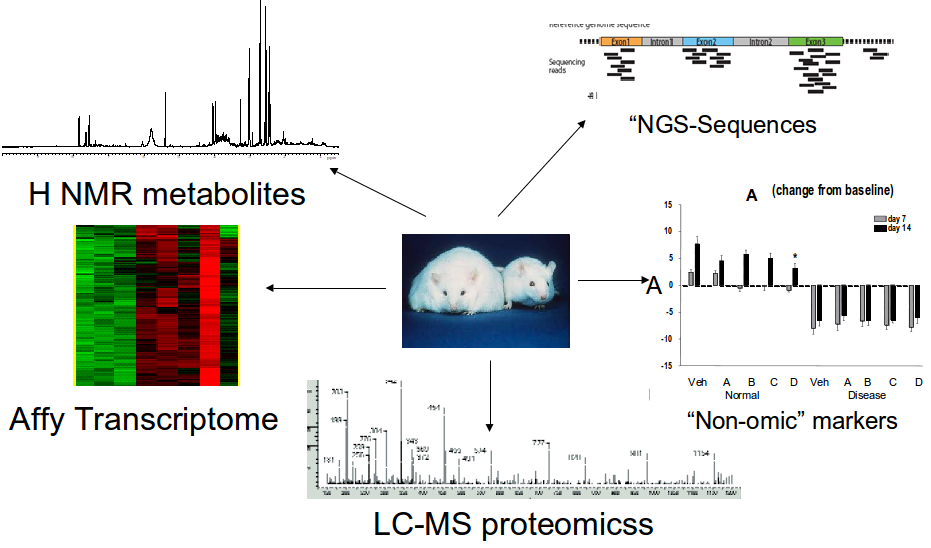
\includegraphics[width=0.6\textwidth]{./images/multipleOmics.png}
\end{itemize} % ends low level

\end{itemize} % ends low level
\end{frame}

\begin{frame}
\frametitle{Data integration and systems biology -again}
\label{sec-1-5}
\begin{itemize}

\item Altogether this opens many fronts and opportunities
\label{sec-1-5-1}%
\begin{itemize}
\item Statistics and bioinformatics are faced with the need for developing methods and tools for the for integrative analysis of big data sets of different sources and types
\label{sec-1-5-1-1}%
\item Biology and medicine are faced with the problem to pose the problems and use the results to improve their understanding in real systems biology approach.
\label{sec-1-5-1-2}%
\end{itemize} % ends low level
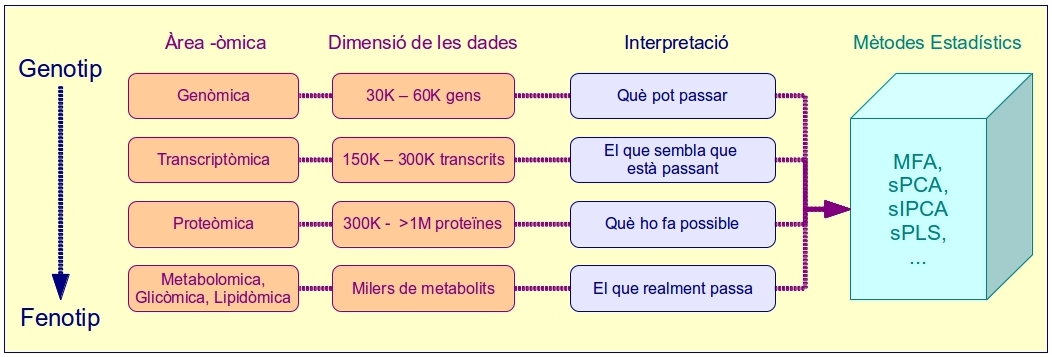
\includegraphics[width=0.9\textwidth]{./images/theOmicsCascade.png}
\end{itemize} % ends low level
\end{frame}

\begin{frame}
\frametitle{Epigenetics and epigenomics}
\label{sec-1-7}
\begin{columns}
\begin{column}{.5\linewidth}
\begin{itemize}
\item Epigenetics, \emph{the study of environmental factors on gene expression in DNA}, shows a renewed impetus:
\label{sec-1-7-1}%
\begin{itemize}
\item NGS allows in-deep analysis of regulatory mechanisms such as \emph{methylation} or \emph{histone modifications}.
\label{sec-1-7-1-1}%
\item There is increasing evidence that many differentiation processes are triggered and maintained through epigenetic mechanisms.
\label{sec-1-7-1-2}%
\end{itemize} % ends low level
\end{itemize} % ends low level
\end{column}
 \begin{column}{.5\linewidth}
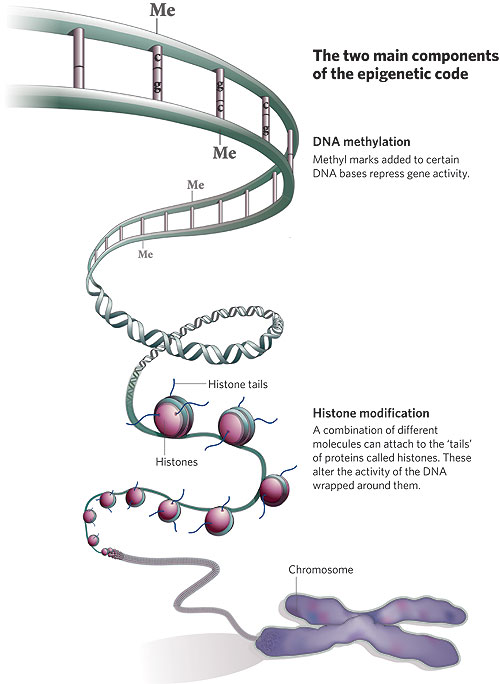
\includegraphics[width=0.9\textwidth]{./images/epigeneticsMechanisms.jpg}
 \end{column}
\end{columns}
\end{frame}

\begin{frame}[fragile]\frametitle{Methylation}
\label{sec-1.8}
\begin{itemize}
\item One main epigenetic regulatory mechanisms is methylation a process by which a gene's behavior is altered, but the gene itself isn't changed.\\
\label{sec-1.8.1}
\item Essentially methylation acts by inhibiting gene expression that is, the more methylated is a gene the more repressed is its expression\\
\label{sec-1.8.2}
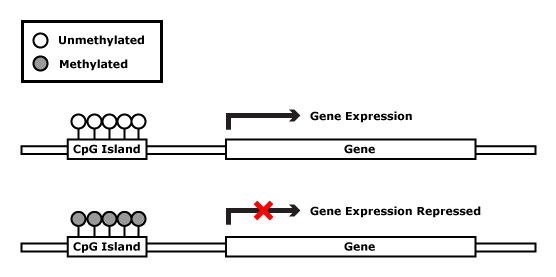
\includegraphics[width=0.7\textwidth]{./images/methylationAction1.png}
%\item Methylation is seen however as a dual phenomenon\\
%\label{sec-1.8.3}
%\begin{itemize}
%\item A methylated gene is "off"\\
%\label{sec-1.8.3.1}
%\item An unmethlated gene is "on"\\
%\label{sec-1.8.3.2}
%\end{itemize} % ends low level
%\item So in practice an important practical problem is to determine at which methylation level a gene is seen as "methylated" (that is turned off).\\
%\label{sec-1.8.4}
\end{itemize} % ends low level
\end{frame}

\begin{frame}[fragile]\frametitle{Methylation and gene expression}
\label{sec-1.8}
\begin{itemize}
\item Although the relation between methylation and gene expression is probably continuous ("\emph{the more...the less...}"), 
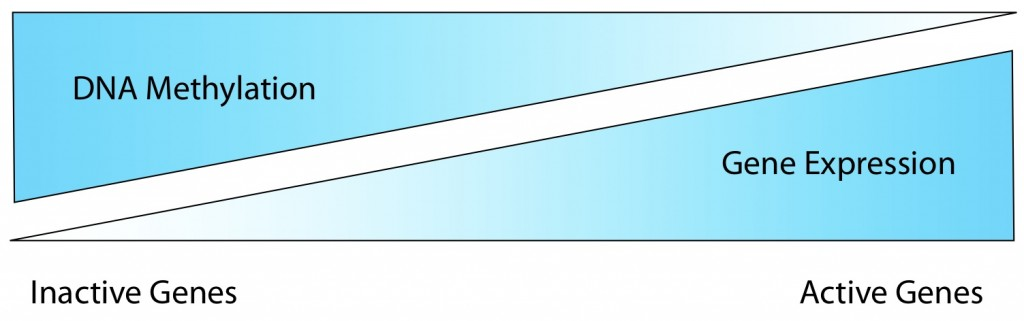
\includegraphics[width=0.7\textwidth]{./images/DNA-Methylation-and-Gene-Expression-Relationship.jpg}
\item methylation is, in practice, seen as a dual phenomenon\\
\label{sec-1.8.3}
\begin{itemize}
\item A methylated gene is "off"\\
\label{sec-1.8.3.1}
\item An unmethlated gene is "on"\\
\label{sec-1.8.3.2}
\end{itemize} % ends low level
\item Practical problem: \textbf{\emph{at which methylation level a gene is seen as "methylated" (that is, it is ``turned off'')?}}
\label{sec-1.8.4}
\end{itemize} % ends low level

\end{frame}

\begin{frame}{Gene-specific methylation on-off threshold}
\begin{itemize}
\item Since measurements for methylation and expression are both
continuous, a biaxial plot of these two signals will exhibit an
L-shape pattern. 
\item If we truly
believe that methylation is binary, there are two implications:
\begin{enumerate}
\item the reflection point of the L-shape is an appropriate choice
to binarize methylation data, and
\item conditioning on the
binarized on-off methylation status, the continuous valued
methylation data and expression data should be independent,
\end{enumerate}
which motivates Liu(2012) to quantify the L-shape pattern using
conditional mutual information (MI). 
\end{itemize}
\end{frame}

\subsection{Motivation}
\begin{frame}{A colon cancer study}
  \begin{itemize}
  \item This study originates in a work searching for colon cancer biomarkers.
  \item 30 cell lines characterized by increasing sensitivity to a drug were analyzed using several high-throughput methods:\emph{ transcriptomics, methylation, miRNAs, SNPs}, and \emph{proteomics}.
\item In this work we consider the problem of stablishing which genes were regulated by methylation.
\item For each gene/methylation locus one has 30 points and a scatterplot showing the relation so we need methods to find patterns of scatterplots
  \end{itemize}
\end{frame}

\begin{frame}{Scatterplot patterns}
\end{frame}



\subsection{Objectives}

\begin{frame}[fragile]\frametitle{Objectives}
\label{sec-1.10}
\begin{itemize}
\item Study how gene expression is regulated by methylation in a set of colon cancer cell lines.\\
\label{sec-1.10.1}
\item Set up a method to detect the level of methylation at which a gene can be considered regulated by methylation (to be "on").\\
\label{sec-1.10.2}
\item Compare this method with other existing that have been developed to\\
\label{sec-1.10.3}
\begin{itemize}
\item detect methylation thresholds\\
\label{sec-1.10.3.1}
\item detect patterns in scatterplots\\
\label{sec-1.10.3.2}
\end{itemize} % ends low level
\end{itemize} % ends low level
\end{frame}



\section{Methods for pattern selection}

\subsection{Based on Conditional Mutual Information}

\begin{frame}{Conditional Mutual Information}
Two questions: which genes exhibit
L-shape, and what is the optimal threshold for binarizing
methylation data for each L-shape gene.
\begin{block}{The key}
To determine whether methylation and expression of a gene exhibit an L-shape,
we compute the conditional Mutual Information (MI) for different choices of threshold
to binarize the methylation data.
\end{block}
If we consider the continuous valued methylation and expression data as two random variables
$X$ and $Y$, and denote a nominal threshold as $t$, the conditional MI can be written as a
weighted sum of MIs on the two sides of the threshold.
\[
\mathit{cMI}(t)=I(X,Y|X>t)P(X>t) + I(X,Y|X\le t)P(X\le t)
\]
\end{frame}

\begin{frame}{Optimal threshold}
When $t$ is $0$ or $1$, $\mathit{cMI}$ equals to the mutual information derived 
from all data points.

For an L-shape gene, as $t$ moves from 0 to 1, $\mathit{cMI}(t)$ first decreases and then
increases, and its value approaches zero when $t$ coincides with the reflection point. 
Therefore,
\begin{block}{Optimal threshold}
The ratio $r=\frac{\min\{\mathit{cMI}(t)\}}{\mathit{cMI}(0)}$ for an L-shape gene is small, 
and $t^{\ast} = \mathrm{argmin}\{ \mathit{cMI}(t) \}$ is the optimal threshold for 
dichotomizing the methylation data of this gene.
\end{block}

\end{frame}

\begin{frame}{Joint distribution estimator}
To estimate the MI terms we use a kernel-based estimator, which constructs a joint
probability distribution by applying a Gaussian kernel to each data point, and estimates
the MI based on the joint distribution. The estimator is as follows:
\[
I(X,Y) = \frac 1M \sum_{i=1}^M \log\frac{M\sum_{j=1}^M e^{-\frac{1}{2h^2}((x_i-x_j)^2+(y_i-y_j)^2)}}{%
                                      \sum_{j=1}^M e^{-\frac{1}{2h^2}(x_i-x_j)^2} \sum_{j=1}^M e^{-\frac{1}{2h^2}(y_i-y_j)^2}}
\]
where $h$ is a tuning parameter for the kernel width and empirically set $h=0.3$.
% i and j are indices for samples.
% In our analysis, we normalize the expression data to zero mean.
\end{frame}

\subsection{Based on Spline regression}


\begin{frame}{Clustering using Spline regression }
We implemented regression based on  $B$-splines because they are particularly efficient due to the block-diagonal basis matrices that result.

Let 
\begin {itemize}
\item $\varsigma=\lbrace t_1 < \ldots < t_N \rbrace$ non decreasing  knot sequence 
\item $\left[ t_m,t_{m+1} \right)$ half open interval
\item $B_{mp}$ p-th order polynomial (degree p-1) with finite support over the interval and 0 everywhere else so that  $\sum_{m=1}^{N-p}B_{mp}(x)=1$
\item then  $s(x)=\sum_{m=1}^{N-p}B_{mp}(x)c_m$ 
\end{itemize}
\end{frame}

\begin{frame}{Clustering using Spline regression (2)}
To represent the curve we set:
\[
y_{ij}=s(x_{ij})
\]
So
\[ 
\mathbf{y}_i=\mathbf{B}_i\mathbf{c}
\]
with
\begin {itemize}
\item $\mathbf{B}_i=\left[ B_{1p}\mathbf{x}_i,B_{2p}\mathbf{x}_i,\dots,B_{Lp}\mathbf{x}_i \right]$ the spline basis matrix
\item $\mathbf{c}$ the vector of spline coefficients.
\end{itemize}
\end{frame}

\begin{frame}{Clustering using Spline regression (3)}
Algorithm
\begin {enumerate}
\item Selection of the genes with a negative significant correlation
\item Fit cubic regression splines
\item Data to cluster: splines coefficients
\item Calculation of a distance matrix between genes as $1-\rho$
\item Hierarchical clustering 
\end{enumerate}
\end{frame}

\section{Results}

\begin {frame}{Results (1) Splines--based regression}
\begin {itemize}
\item After the previous selection of genes we worked with 292 genes
\item We decided to choose 5 clusters
\item The 2 first clusters included the genes with an L-shape
\end{itemize}
\end{frame}

\begin{frame}{Results (2) Conditional Mutual Information}
\begin {itemize}
\item No previous selection of the genes was needed
%\begin{block}{Three criteria}
\item We filtered for L-shapes using a combination of three criteria:
\begin{itemize}
\item the ratio $r<0.25$
\item unconditioned MI $\mathit{cMI}(0)>0.1$
\item the median expression on the left side of the optimal threshold $t^{\ast}$ is higher
than the median expression on the right side.
\end{itemize}
%\end{block}
\item The parameters are chosen according to a random permutation test (see Liu(2012)).
\item According to the above criteria, a total of 641 genes are selected to be L-shape genes.
\end{itemize}
\end{frame}


\begin{frame}{Results (3) Comparison between the methods}
The results of both methods that can be summarized in the following table:
\begin{center}
\begin{tabular}{|c|c|c|}
\hline
Cluster & Splines & cMI \\
\hline
1 & 140 & 102 \\
2 & 22 & 16 \\
\hline
Total & 162 & 118 \\
\hline
\end{tabular}
\end{center}
\end{frame}

\begin{frame}{Conclusions}
  \begin{itemize}
  \item We have found similar results between both methods.
  \item Biological interpretation is still being done by biological
    researchers although results are consistent with the hypothesis
    (we have found genes regulated by methylation).
  \item Sample size is a limiting factor: cMI works better with hundreds of samples but one may have a very small number (real cases: 30, 12)
\end{itemize}
\end{frame}

\begin{frame}{Acknowledgments}
  \begin{itemize}
  \item 
  \end{itemize}
\end{frame}



\end{document}
